\chapter{ Констукторский раздел}
\label{cha:design}
    В данном разделе будут рассмотрены схемы алгоритмов, требования к функциональности ПО, и определены способы тестирования.
    
    \section{Описание структур данных}
        Муравьиная колония представляет собой структуру данных, которая содержит информацию об абстракциях, представленных ниже.
        \begin{enumerate}
            \item Граф, с которым будет работать алгоритм. Сам граф представлен матрицей смежности.
            \item Матрицу феромонов, содержащую количество феромона в каждом узле.
            \item Количество дней, которое «проживет» колония.
            \item Конфигурационную структуру, содержащую регулируемые параметры, описанные в разделе \ref{cha:analytical}.
        \end{enumerate}
        Муравей -- структура, содержащая информацию о типе муравья, колонии, начальную и текущую позицию и матрицы пройденного пути и запретных городов. Матрицу запретных городов было решено заполнить логическими значениями. Матрица пройденного пути содержит расстояния между двумя соответствующими узлами.
    \section{Описание памяти, используемой алгоритмом}

\subsection{Алгоритм полного перебора}
Оценка памяти рекурсивного алгоритма сводится к подсчету количества рекурсивных вызовов и объема работы, выполняемого для каждого вызова. В данном случае расчет производится по формуле \ref{math:mem-rec}:
\begin{equation}\label{math:mem-rec}
    \begin{array}{c}
        M_{brute} = \left(\left(n \cdot lvar_{prem} + ret\right) \cdot depth + m \cdot lvar\right) \cdot \\
        |graph| + size_{int} \cdot |graph|
    \end{array}
\end{equation}
где $depth$ -- глубина стека вызовов, равная количеству перестановок при нахождении полного перебора, $|graph|$ -- размер матрицы смежности, $lvar_{prem}$ -- размер аллоцированных переменных в рекурсивной части функции и $n, m$ -- их количество. Аналогично, $lvar$ -- размер аллоцированных в итеративной части функции. Выражение $size_{int} \cdot |graph|$ определяет размер временного массива для хранения текущего пути.

\subsection{Муравьиный алгоритм}
Память, используемая муравьиным алгоритмом, складывается из содержимого структуры колонии и содержимого структуры каждого муравья. Таким образом, формула принимает вид \ref{math:mem-ant}:
\begin{equation}\label{math:mem-ant}
    \begin{array}{l}
    M_{ant-alg} = |graph| \cdot M_{ant} + M_{colony}, \text{ где:} \\
    M_{ant} = \left(size_{int} \cdot |graph|\right)^2 + \left(size_{bool} \cdot |graph|\right)^2 + 2 \cdot size_{int} + \\
    + ptr\left(M_{col}\right), \\
    M_{col} = \left(size_{int} \cdot |graph|\right)^2 + \left(size_{float} \cdot |graph|\right)^2 + size_{int} + \\
    + k \cdot size_{float}
    \end{array}
\end{equation}
Здесь $M_{ant}$ -- размер памяти используемый каждым муравьем в колонии, $M_{col}$ -- размер памяти, используемый колонией, $ptr\left(M_{col}\right)$ -- размер указателя на структуру колонии. Остальные обозначения аналогичны \ref{math:mem-rec}.
	
	\section{Схемы алгоритмов}
        Ниже будут представлены схемы алгоритмов: \begin{enumerate}
            \item муравьиного алгоритма (рисунки \ref{fig:ant}, \ref{fig:ant-wheel}, \ref{fig:ant-phero});
            \item алгоритма полного перебора (рисунок \ref{fig:brute}).
        \end{enumerate}

\begin{center}
    \begin{figure}[!h]
        \centering
        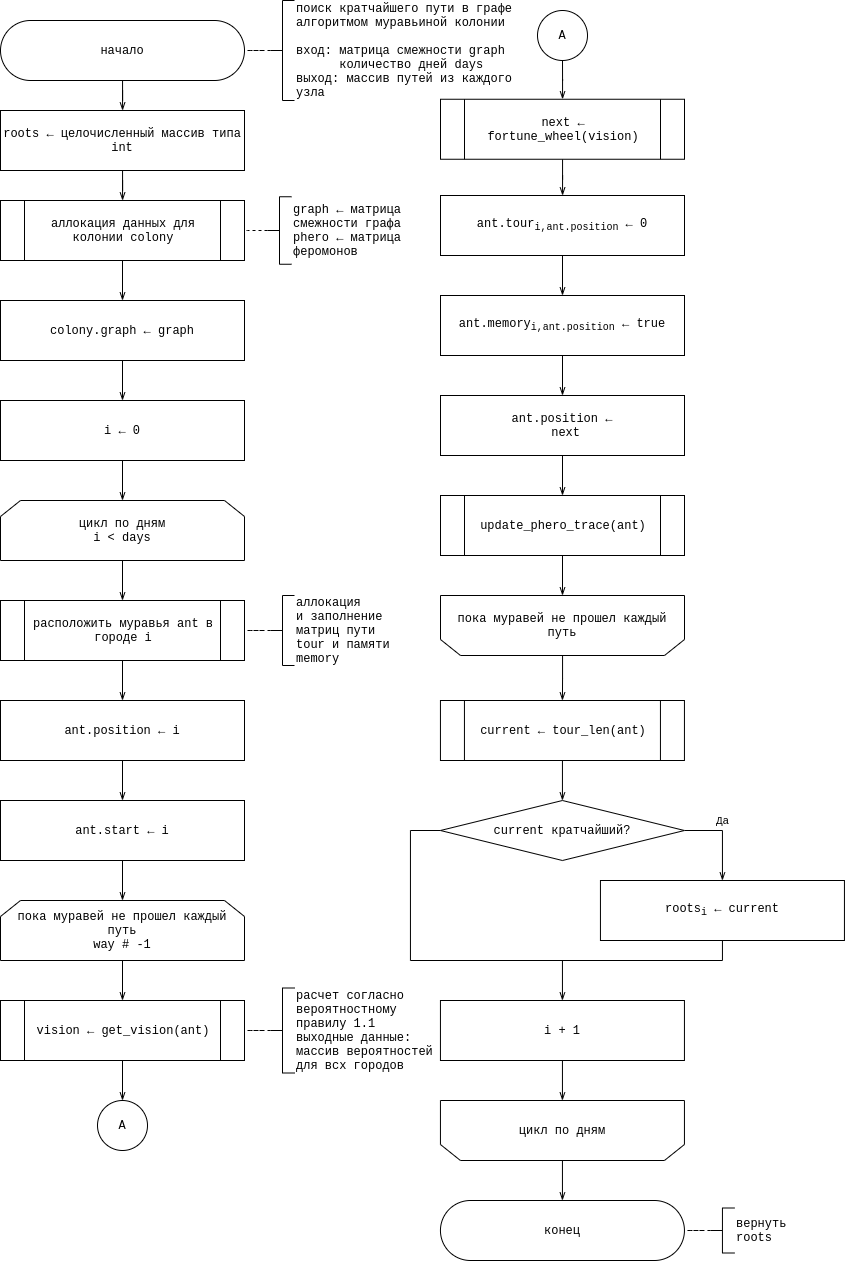
\includegraphics[width=0.85\linewidth]{img/tsp-ant.drawio.png}
        \caption{Схема работы муравьиного алгоритма}
        \label{fig:ant}
    \end{figure}
\end{center}
\newpage


\begin{center}
    \begin{figure}[!h]
        \centering
        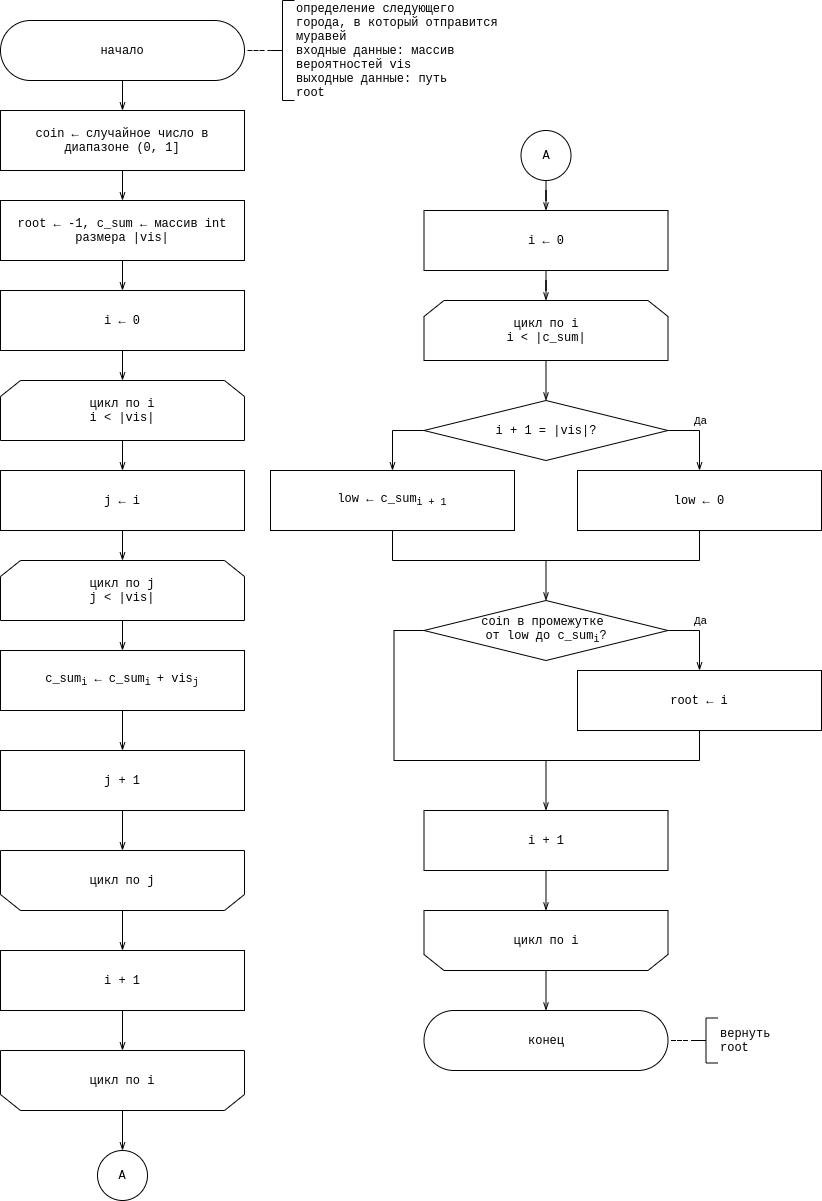
\includegraphics[width=0.85\linewidth]{img/tsp-ant-wheel.drawio.png}
        \caption{Схема работы алгоритма случайного выбора города}
        \label{fig:ant-wheel}
    \end{figure}
\end{center}
\newpage

      \begin{center}
    \begin{figure}[!h]
        \centering
        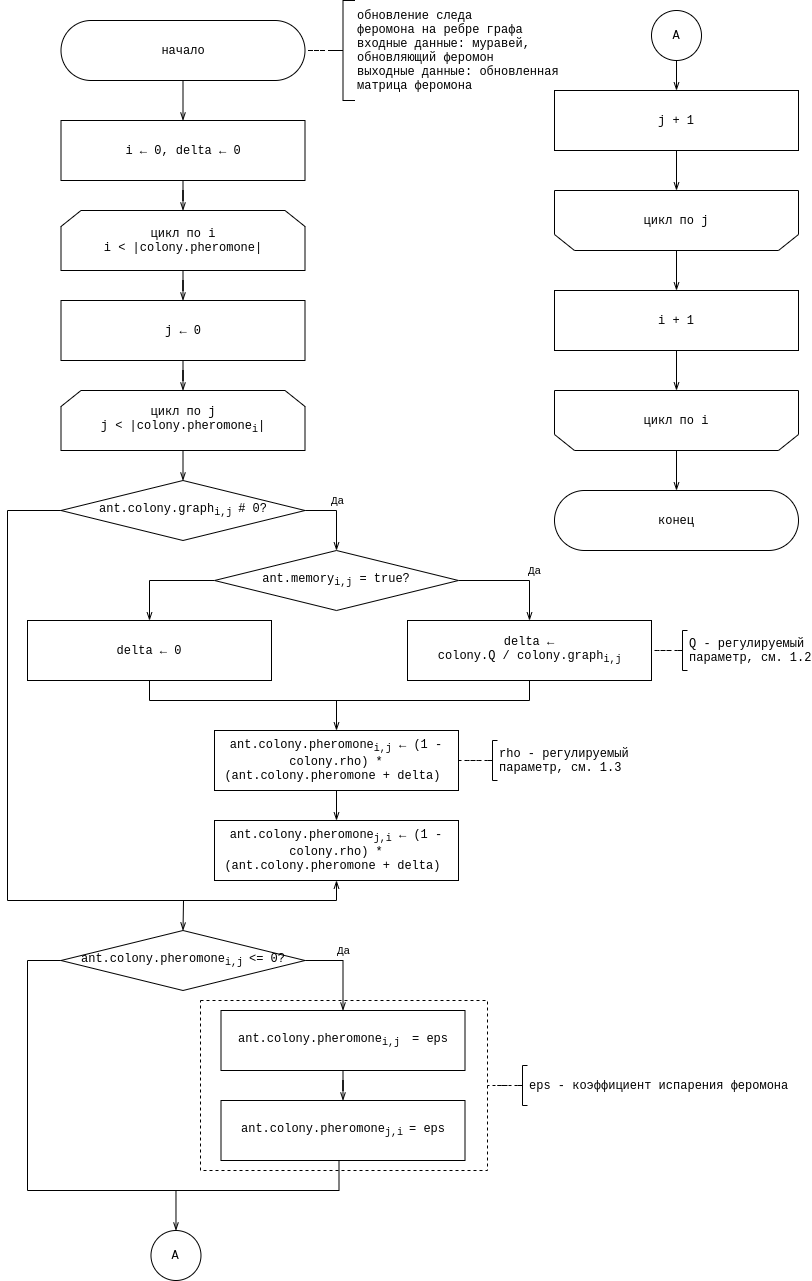
\includegraphics[width=0.8\linewidth]{img/tsp-phero.drawio.png}
        \caption{Схема работы алгоритма обновления феромона}
        \label{fig:ant-phero}
    \end{figure}
\end{center}
\newpage

\begin{center}
    \begin{figure}[!h]
        \centering
        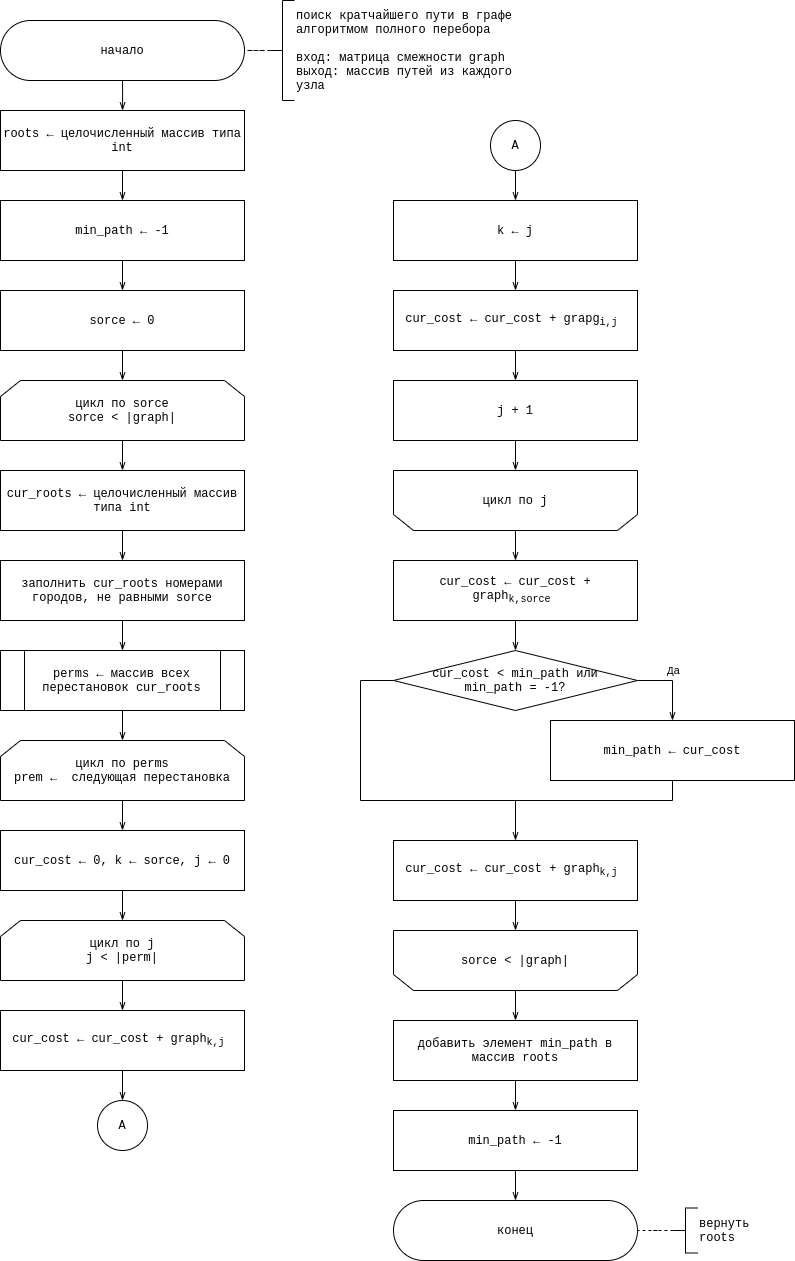
\includegraphics[width=0.87\linewidth]{img/tsp-brute.drawio.png}
        \caption{Схема работы алгоритма "грубой силы"}
        \label{fig:brute}
    \end{figure}
\end{center}
\newpage
\text{   }
        

    \section{Структура ПО}
    \par Программа поделена на ряд смысловых модулей, описанных ниже:
    \begin{itemize}
        \item Модуль «brute», в котором содержится реализация алгоритма полного перебора;

        \item Модуль «aco», в котором содержится реализация алгоритма муравьиной колонии;

        \item Модуль «interf», в котором содержатся вспомогательные функции для пользовательского интерфейса.
    \end{itemize}

    Программа имеет консольный интерфейс.

	\section*{Вывод}
    \par Были разработаны схемы алгоритмов, необходимых для решения задачи. Получено достаточно теоретической информации для написания программного обеспечения.
\newpage